\documentclass[UTF8]{ctexbeamer}	% Compile at least twice!
%\setbeamertemplate{navigation symbols}{}
\usetheme{Madrid}
% \setbeamertemplate{navigation symbols}{}
% \useinnertheme{rectangles}
% \useoutertheme{infolines}
% \useoutertheme[title,section,subsection=true]{smoothbars}
\useoutertheme{split}
\useinnertheme{rounded}
\setbeamertemplate{headline}{}
\usecolortheme{beaver}


% \usecolortheme{default}
% \usecolortheme{whale}
 
% -------------------
% Packages
% -------------------
\usepackage{
    amsmath,			% Math Environments
    amssymb,			% Extended Symbols
    enumerate,		    % Enumerate Environments
    graphicx,			% Include Images
    lastpage,			% Reference Lastpage
    multicol,			% Use Multi-columns
    multirow,			% Use Multi-rows
    pifont,			    % For Checkmarks
    stmaryrd,            % For brackets
    listings,
    subfigure,
}
\usepackage[english]{babel}
\usepackage{graphicx}
\usepackage{animate}
\usepackage{xeCJK}
\usepackage{fontspec} 
% \setsansfont{Times New Roman}
% \setmonofont{Times New Roman}
\setmainfont{Times New Roman Cyr}
\setCJKmainfont{方正新楷体简体}

\newfontfamily\os{Open Sans}
\newfontfamily\oscl{Open Sans Condensed}
\newfontfamily\tnr{Times New Roman}
\newfontfamily\tnrc{Times New Roman Cyr}
\newfontfamily\tim{Times}
\newfontfamily\roc{Rockwell}
% \usepackage{CJK}
% \lstset{language=C++}
% \lstset{extendedchars=false}
% \lstset{breaklines}


% -------------------
% Colors
% -------------------
% \definecolor{UniOrange}{RGB}{212,69,0}
% \definecolor{UniGray}{RGB}{62,61,60}
% \definecolor{UniRed}{HTML}{B31B1B}
% \definecolor{UniGray}{HTML}{222222}
% \setbeamercolor{title}{fg=UniGray}
% \setbeamercolor{frametitle}{fg=UniOrange}
% \setbeamercolor{structure}{fg=UniOrange}
% \setbeamercolor{section in head/foot}{bg=UniGray}
% \setbeamercolor{author in head/foot}{bg=UniGray}
% \setbeamercolor{date in head/foot}{fg=UniGray}
% \setbeamercolor{structure}{fg=UniOrange}
% \setbeamercolor{local structure}{fg=black}
% \beamersetuncovermixins{\opaqueness<1>{0}}{\opaqueness<2->{15}}


% -------------------
% Fonts & Layout
% -------------------
% \usepackage{palatino}
\usefonttheme{serif}
% \setbeamerfont{title like}{shape=\scshape}
% \setbeamerfont{frametitle}{shape=\scshape}
% \setbeamertemplate{itemize items}[circle]
% \setbeamertemplate{enumerate items}[default]


% -------------------
% Commands
% -------------------

% Special Characters
% \newcommand{\N}{\mathbb{N}}
% \newcommand{\Z}{\mathbb{Z}}
% \newcommand{\Q}{\mathbb{Q}}
% \newcommand{\R}{\mathbb{R}}
%\newcommand{\C}{\mathbb{C}}

% Math Operators
% \DeclareMathOperator{\im}{im}
% \DeclareMathOperator{\Span}{span}

% Special Commands
% \newcommand{\pf}{\noindent\emph{Proof. }}
% \newcommand{\ds}{\displaystyle}
% \newcommand{\defeq}{\stackrel{\text{def}}{=}}
% \newcommand{\ov}[1]{\overline{#1}}
% \newcommand{\ma}[1]{\stackrel{#1}{\longrightarrow}}
% \newcommand{\twomatrix}[4]{\begin{pmatrix} #1 & #2 \ #3 & #4 \end{pmatrix}}


% -------------------
% Tikz & PGF
% -------------------
\usepackage{tikz}
\usepackage{tikz-cd}
\usetikzlibrary{
    calc,
    decorations.pathmorphing,
    matrix,arrows,
    positioning,
    shapes.geometric
}
\usepackage{pgfplots}
\pgfplotsset{compat=newest}
\usepackage{wrapfig}
\usepackage{cite}


% -------------------
% Theorem Environments
% -------------------
\usepackage{amsthm}
\theoremstyle{plain}
\newtheorem{sit}{Situation}[section]
\newtheorem{prop}{Proposition}[section]
\newtheorem{rtm}{Theorem}[section]
\newtheorem{cor}{Corollary}[section]
\theoremstyle{definition}
\newtheorem{das}{Data structure}[section]
\newtheorem{nex}{Non-Example}[section]
\newtheorem{cla}{class}[section]
\newtheorem{emt}{}[section]
\newtheorem{defn}{Definition}[section]
\theoremstyle{remark}
\newtheorem{rem}{Remark}[section] 
\numberwithin{equation}{section}

\newcommand\caesura{$\mkern -8.5mu\raise -.2ex\hbox{\rotatebox[]{180}{\`}}\ $}
\setbeamertemplate{caption}[numbered]
% -------------------
% Title Page
% -------------------
\title{\textcolor{red}{2022年硕博连读面试}}
%\subtitle{\textcolor{white}{Mathematics Conference for the Mysterious and dMagical}}  
\author{申请人: 谭焱 
% \newline \newline
%  \small{硕士导师: 王何宇\, \
%  申请博士导师: 张庆海}
 }

\institute{\small{现硕士导师: 王何宇 、张庆海 \newline 拟转博士指导教师: 张庆海} \newline   \newline 浙江大学数学科学学院}
\date{\today} 


% -------------------
% Content
% -------------------
\begin{document}

% Title Page
\begin{frame}
  \titlepage
\end{frame}


\begin{frame}
  \frametitle{提纲}
  \tableofcontents
\end{frame}

\begin{frame}
  老师们下午好,我是王何宇老师和张庆海老师联合培养的硕士生谭焱,今天在这里向
  各位专家教授做硕转博申请报告,申请的博士指导教师是张老师,
  接下来介绍一下硕士期间的学习和科研经历.
\end{frame}

\begin{frame}
  我今天要讲的分为三部分,简单说明一下个人基本情况后着重介绍我的科研工作,
  硕士期间,张老师安排我做一个涉密项目,由于涉密原因不能对项目完整赘述.
  今天讲的是我们为完成项目进行的理论铺垫--殷集和布尔代数.最后说一下我计划
  博士期间如何将殷集应用到军工项目中.
\end{frame}

\begin{frame}
  在修习学分的时候学习了做科研需要的基础知识和英文阅读写作能力.同时也
  针对性训练了科研工作需要的能力,例如编程和图形学可视化等.
\end{frame}

\begin{frame}
  然后是我的科研工作,潜艇在海底航行会在海面上产生一些特殊的波纹,
  我们期望通过计算有潜艇表面和海水表面两个动边界的方程,
  从而实现对潜艇的追踪和反追踪.我的主要工作在对动边界的追踪同时提取
  拓扑和几何信息上.
\end{frame}

\begin{frame}
  就像刚说的潜艇项目,军工领域中有动边界的流体方程计算是重要研究课题.现有方法比如
  vof方法,ft方法还有水平集法
  在界面追踪的时候将几何和拓扑问题转化为求解微分方程,简化了理论和计算复杂度
  也导致了一些问题,比如这里说到的四点,特别是对动流场的拓扑信息的捕捉.
  张庆海教授的想法是用几何和拓扑的手段处理界面追踪这个几何和拓扑的问题.
  第一步是对动流相几何建模.
  2020年张庆海教授和黎至轩学长提出了二维殷集给二维空间中的流相建模.
\end{frame}

\begin{frame}
  那殷集和布尔代数和几何和拓扑有什么关系呢?用殷集建模有什么好处呢?
  可以从殷集的简单表示中快速提取拓扑信息,
  殷集建模保留了界面上拓扑信息,所以支持界面追踪的高保真算法,
  布尔代数给刻画动流相的拓扑变化提供了核心工具.
  % 殷集为流相提供了简单表示,从表示中可以直接得出欧拉示性数
  % 等拓扑不变量,比如连通分量数和闭包的洞的数量.并且因为殷集保留了界面上的拓扑信息,
  % 可以实现界面追踪的高保真算法,殷集上的布尔运算是研究流相拓扑变化的
  % 核心工具,从理论上支持刻画多相流的拓扑变化
  .综上殷集和布尔代数用几何和拓扑的手段解决界面追踪问题,是我们
  研究潜艇项目中至关重要的一步.
\end{frame}

\begin{frame}
  先给出殷集的数学定义,殷集是空间中边界有界的半解析开集.
  有界和解析性是因为计算只有有限的计算资源,只能考虑有限的显示信息,比如
  没有解析性的两个正则开集的布尔求交可能得到无穷多个连通域.而
  正则性捕捉了流相连续的本质.
  先来看二维空间中的殷集,在已发表论文中我们提供并
  证明了这个二维殷集的简单表示
  ,并高效实现了布尔代数.如图中熊猫和
  米老鼠求交运算后的殷集结果.其中黄色区域是殷集内部,其余是外部.
  % 我希望从二维类推到三维空间中
  % ,公式表达中可以发现关键在于每个连通分量的边界.
  从二维殷集的唯一表示中不难发现关键在于连通分量的边界,二维是约当曲线,
\end{frame}

\begin{frame}
  我们在三维空间中寻找可以合适表达殷集边界的数学概念.这时二流形分类定理
  走入视线,但这还不够,如图中常见的三维区域中可能存在非流行点,因此考虑
  将二流形粘起来的黏合紧曲面.
\end{frame}

\begin{frame}
  顺理成章地,类似提供并证明了殷集在三维空间中的高效唯一表示.
  黏合紧曲面代替约当线.如图是一个环面内挖去两个球,此时两个球将环面内部分为
  两个不连通的开集.所以殷集y有两个联通分量,
  表示殷集y的边界是两个对称的同胚于圆柱的黏合紧曲面,
  而不是两个球和一个环面.
  我们证明了每个内部有界的黏合紧曲面对应一个连通分量,
  每个内部无界的黏合紧曲面对应殷集闭包的一个洞.
\end{frame}

\begin{frame}
  有了简单表示后,再来实现布尔代数来捕捉拓扑变化.实现过程大致分五步,
  计算非流形点,将黏合紧曲面剪开,处理曲面片,最后粘起来唯一表示结果殷集.
  % 首先直接计算殷集边界的非流形点,沿非流形点将边界剪开得到曲面片,然后
  % 处理曲面片,比如如果是求补运算,只需要改变每个曲面片的方向,交需要移除
  % 部分曲面片.最后将处理过的曲面片重新黏合成合适的黏合紧曲面唯一表示
  % 一个殷集作为布尔运算的结果.
  下面以殷集1,2交并结果作为示范说明这个过程.y1是之前说的一个环内
  挖去两个球,y2是略大一圈的球,恰好包含了y1右边的小球.
\end{frame}

\begin{frame}
  计算非流行点并将黏合紧曲面剪开得到曲面片,注意因为是两个殷集求交,
  y2把y1剪开的曲面片分为两部分,分别是在y2内部和外部的曲面片
  ,类似的y2被y1切出两个圆片在y1内,剩余的在y1外.
  当求交时,移除不在另一个殷集内部的曲面片,如图a中移除了左边的半球面和长的柱面,
  b中保留了两个圆盘.然后将曲面片沿非流行点构成的边界粘起来
  得到d中的黏合紧曲面表示c中的y3.
\end{frame}

\begin{frame}
  求并时保留的曲面片恰好相反,保留在另一个殷集外的曲面片,粘起来的黏合紧曲面如图f所示.
  y3的表示中两个内部有界的黏合紧曲面对应两个连通分量,y4表示
  的一个内部有界一个无界的黏合紧曲面对应一个连通分量一个洞,
  再一次验证了殷集表示和拓扑不变量之间的一一对应关系.
  % 殷集表示中可以迅速得到连通分量数betti数0和洞的数量betti数2.
  对几何特征复杂的殷集处理是容易的,因为我们只在非流行点构成的一维
  CW复形上操作剪切粘贴.
  至此已经实现了三维殷集建模和布尔代数.
\end{frame}

\begin{frame}
  三维殷集工作的论文在写,期望使用三维殷集做出应用后论文
  发表能在二维殷集基础上更上一层.
\end{frame}

\begin{frame}
  之前提到现有方法对拓扑变化
  处理的不足.博士阶段计划应用三维殷集到张庆海教授提出的MARS方法上,实现对
  有拓扑变化的动边界高精度追踪.也是潜艇项目中的动边界不可或缺的一部分.
\end{frame}
% % Motivation
% \section{个人基本情况介绍}

% % Definitions & Examples
% \begin{frame}[fragile]
%     \frametitle{学习情况}
%     \begin{enumerate}
%         \item 研究生课程
%               \begin{itemize}
%                   \item 科研相关课程获得良好成绩
%                         \begin{itemize}
%                             \item 非线性问题的数学方法(92), 图形学的新进展(90) 等.
%                         \end{itemize}
%                   \item 英语阅读及写作方面
%                         \begin{itemize}
%                             \item 六级489分(阅读205)可以流畅阅读英文文献.
%                             \item 通过研究生论文写作指导(92)打下坚实写作基础.
%                         \end{itemize}
%               \end{itemize}
%         \item 科研训练
%               \begin{itemize}
%                   \item 系统地学习了代数拓扑和微分方程数值解的相关理论.
%                   \item 锻炼了算法设计和编程实现能力.
%                   \item 培养了将代数拓扑和微分方程数值解结合进行科学研究的思维方式.
%               \end{itemize}
%     \end{enumerate}
% \end{frame}

% \section{硕士阶段的科研工作}
% \subsection{涉密的军工项目}
% \begin{frame}
%     \frametitle{涉密军工项目}
%     \begin{itemize}
%         \item 潜艇湍流尾迹的海洋表面特征等内波现象的研究, 用于潜艇追踪和隐身
%               (\textcolor{red}{军科委基础加强重点项目}).
%               \begin{figure}
%                   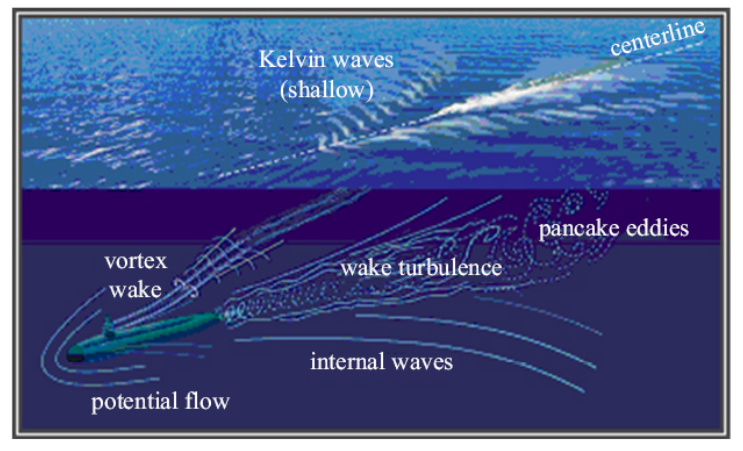
\includegraphics[width = 0.7\textwidth]{fig/s12.png}
%                   \caption{水下潜艇产生的各种尾迹示意图, 包括开尔文尾迹, 内波, 湍流尾迹, 涡尾迹, 煎
%                       饼旋涡.}
%               \end{figure}
%     \end{itemize}
% \end{frame}

% \subsection{\textcolor{red}{非涉密的三维殷集和布尔代数}}
% \begin{frame}
%     \frametitle{殷集的研究背景}
%     \begin{itemize}
%         \item 含有动边界的不可压流体在军工领域是非常重要的研究课题.
%         \item 现有方法是对界面的几何和拓扑问题进行回避,导致了:
%               \begin{enumerate}
%                   \item 对等距变换的流场不能保证几何性质.
%                   \item 对同胚映射的流场不能保证拓扑性质.
%                   \item 精度最高为二阶精度.
%                   \item 很难对拓扑变化进行严格的处理.
%               \end{enumerate}
%         \item 我们的核心思想是用\textcolor{red}{几何和拓扑的手段
%                   研究几何和拓扑的问题},其中首要工作在于对流相建模
%               (Zhang and Li, \tnr{ Math. Comput.}\tnrc{, \ 2020).}

%               %   \os (Zhang and Li 2020 Math. Comput.).

%               %   \oscl (Zhang and Li 2020 Math. Comput.).

%               %   \tnr (Zhang and Li 2020 Math. Comput.).

%               %   \tim (Zhang and Li 2020 Math. Comput.).

%               %   \roc (Zhang and Li 2020 Math. Comput.).
%     \end{itemize}
%     \begin{center}
%         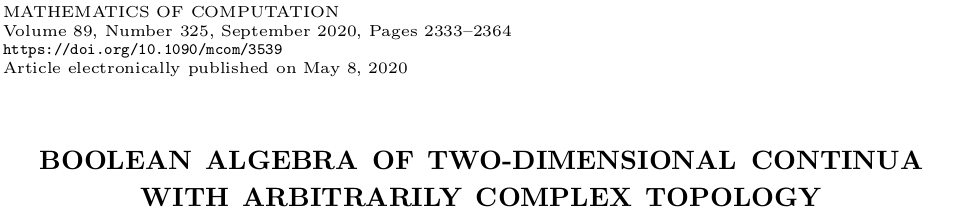
\includegraphics[width = 0.9\textwidth]{fig/s14.png}
%     \end{center}
% \end{frame}


% \begin{frame}
%     \frametitle{殷集和布尔代数的重要性}
%     \begin{itemize}
%         \item 几何和拓扑的手段集中体现在殷空间和布尔代数.
%         \item 为连续介质提供了简单高效的表示(以O(1)时间得到欧拉示性数).
%         \item 给动边界的界面追踪的高保真算法提供理论支撑.
%         \item 给多相流的流相拓扑变化刻画和高阶算法设计提供理论支撑.
%         \item 是许多重大科学问题(军工项目)的核心难点.
%     \end{itemize}

%     \begin{columns}
%         \column{0.5\linewidth}<1->
%         \centering
%         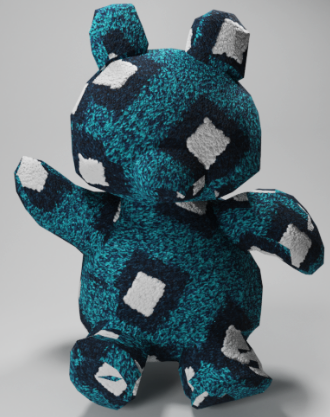
\includegraphics[width = .6\textwidth]{fig/s18.png}
%         \column{0.5\linewidth}<1->
%         \centering
%         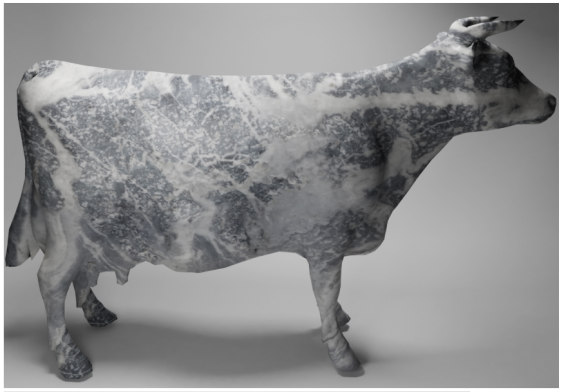
\includegraphics[width = .8\textwidth]{fig/s19.png}
%     \end{columns}
% \end{frame}


% \begin{frame}
%     \frametitle{二维殷集}
%     \begin{itemize}
%         \item 二维空间中,任一个殷集可以唯一表示为
%               \[\mathcal{Y} = \cup_j^{\bot \bot}\cap_i \text{int}(\gamma_{j, i} ),\]
%               约当曲线 $\gamma_{j, i}$是$\mathcal{Y}$内第j$个连通分量
%               的第i$条边界.
%         \item 高效实现了殷集上的布尔代数.
%     \end{itemize}
%     \begin{figure}[htb]
%         \centering
%         \subfigure{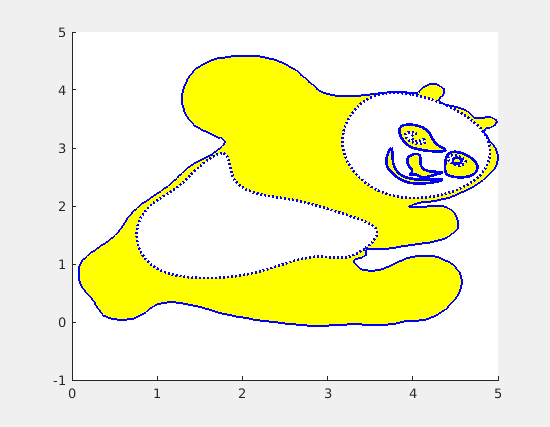
\includegraphics[width=0.3\textwidth]{fig/p.png}}
%         \subfigure{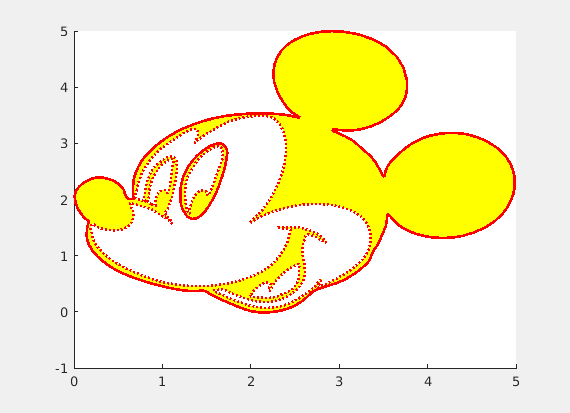
\includegraphics[width=0.3\textwidth]{fig/m.png}}
%         \subfigure{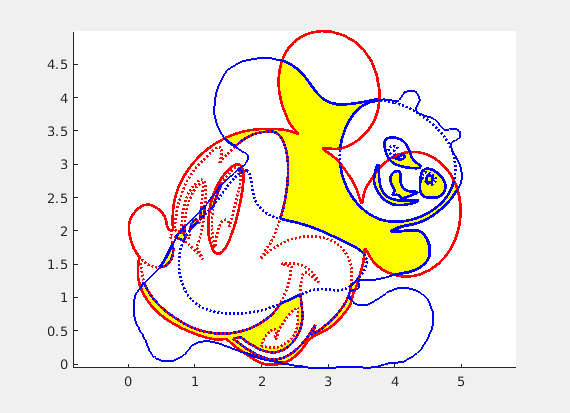
\includegraphics[width=0.3\textwidth]{fig/pm.png}}
%     \end{figure}
% \end{frame}

% \begin{frame}
%     \frametitle{科研成果---三维殷集的数学模型及布尔代数}
%     \begin{itemize}
%         \item
%               \textcolor{red}{二流形的分类定理} \newline
%               有向的紧二流形是同胚于球或者圆环或它们的有限个连通和.
%               \begin{center}
%                   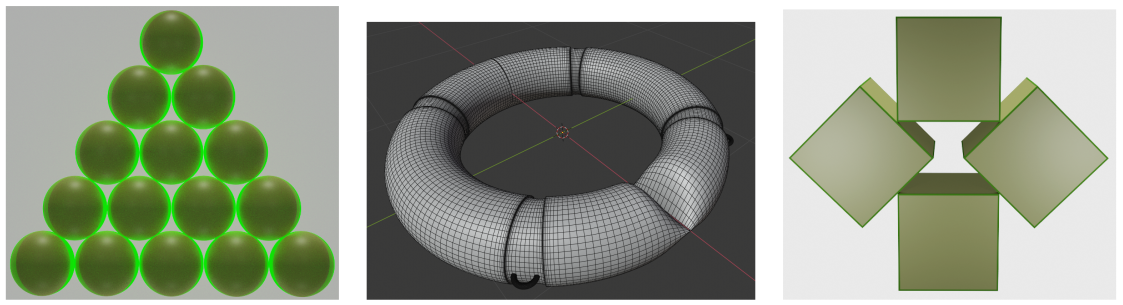
\includegraphics[width = .9\textwidth]{fig/s15.png}
%               \end{center}


%         \item 黏合紧曲面是一个二维连通紧流形或这种流形的商空间, 其商映射
%               将多个与一维 CW 复形同胚的子集粘在一起; 将这个一维子集删除后
%               该黏合紧曲面仍然是连通的.
%     \end{itemize}
% \end{frame}

% \begin{frame}
%     \frametitle{三维殷集的唯一表示}
%     \begin{itemize}
%         \item \textcolor{red}{三维殷集}:三维空间中边界有界的正则半解析开集.所有三维殷集构
%               成的集合被称为殷空间,记为 $\mathbb{Y}$.
%         \item 任一个殷集$\mathcal{Y} \in \mathbb{Y}$可以唯一表示为
%               \[\mathcal{Y} = \cup_j^{\bot \bot} \cap_i \text{int}(\Gamma_{j, i}),\]
%               黏合紧曲面$\Gamma_{j, i}$是$\mathcal{Y}$的第j$个连通分量的第i$个边界.
%     \end{itemize}
%     \begin{figure}[htbp]
%         \centering
%         \subfigure[殷集$\mathcal{Y}$]{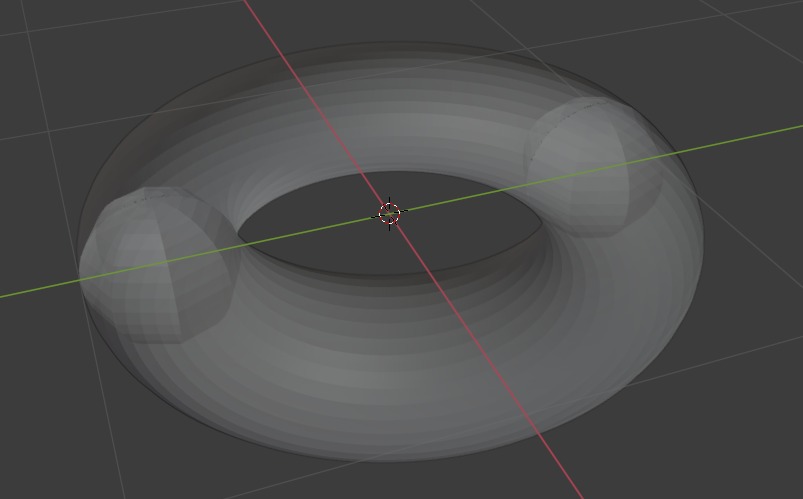
\includegraphics[width=0.4\textwidth]{fig/s1.png}} \qquad
%         \subfigure[表示$\mathcal{Y}$的两个黏合紧曲面]{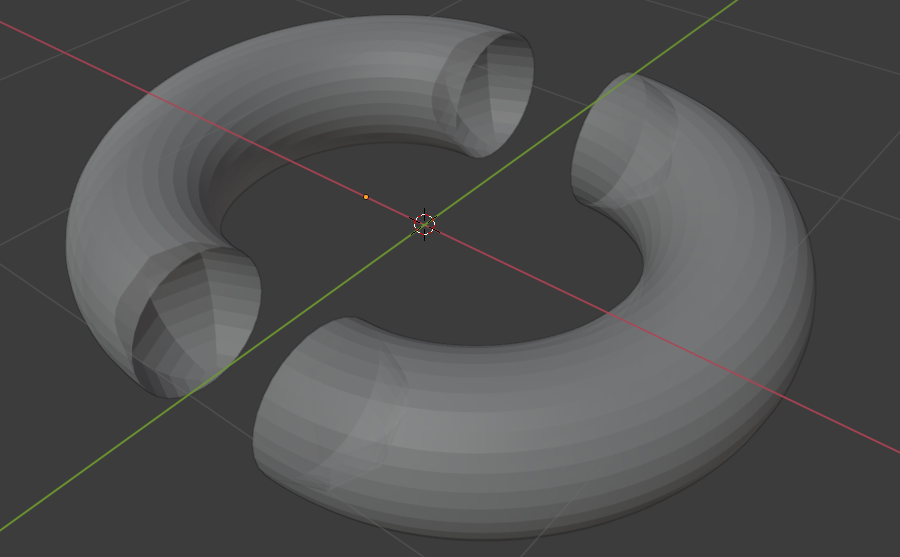
\includegraphics[width=0.4\textwidth]{fig/s2.png}}
%         \caption{殷集和表示殷集的黏合紧曲面}
%         \vspace{0.2in}
%     \end{figure}
% \end{frame}

% \begin{frame}
%     \frametitle{布尔代数的实现方式}
%     \begin{enumerate}
%         \item 计算殷集边界上的所有非流形点.
%         \item 沿非流形点剪开黏合紧曲面得到若干曲面片.
%         \item 根据交并补的需要删除曲面片或改变曲面片方向.
%         \item 将曲面片重新黏合成黏合紧曲面集合.
%         \item 黏合紧曲面集合唯一表示一个三维殷集作为布尔运算结果.
%     \end{enumerate}
%     \begin{figure}[!htb]
%         \centering
%         \subfigure[殷集$\mathcal{Y}_1$]{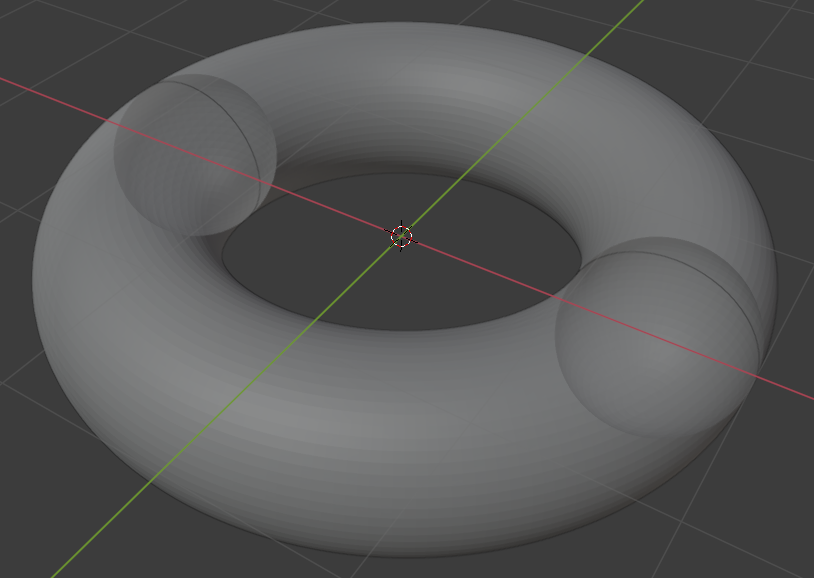
\includegraphics[width=0.365\textwidth]{fig/s3.png}} \qquad
%         \subfigure[殷集$\mathcal{Y}_2$]{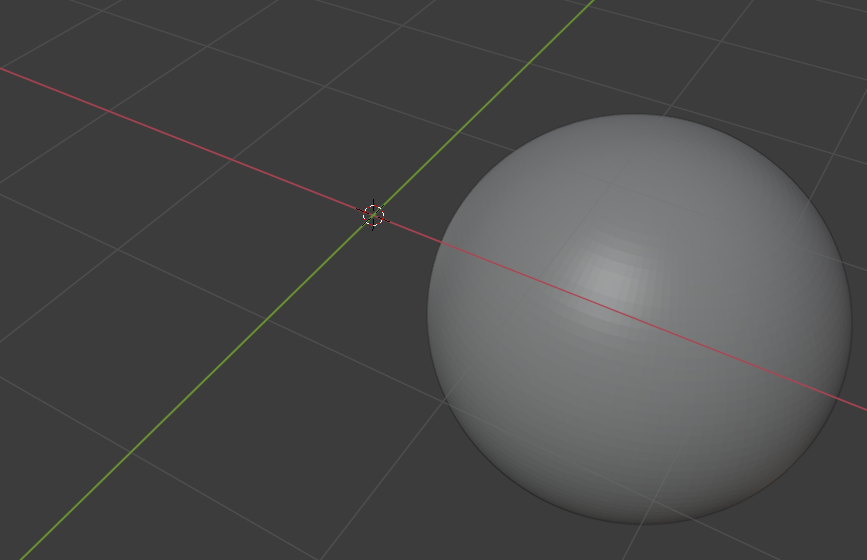
\includegraphics[width=0.4\textwidth]{fig/s4.png}}
%         \caption{将要进行布尔运算的殷集$\mathcal{Y}_1$和$\mathcal{Y}_2$}
%         \vspace{0.2in}
%     \end{figure}
% \end{frame}

% \begin{frame}
%     \frametitle{布尔运算结果图}
%     \begin{figure}[!htb]
%         \centering
%         \subfigure[$\partial\mathcal{Y}_1$剪开得到的部分曲面片]
%         {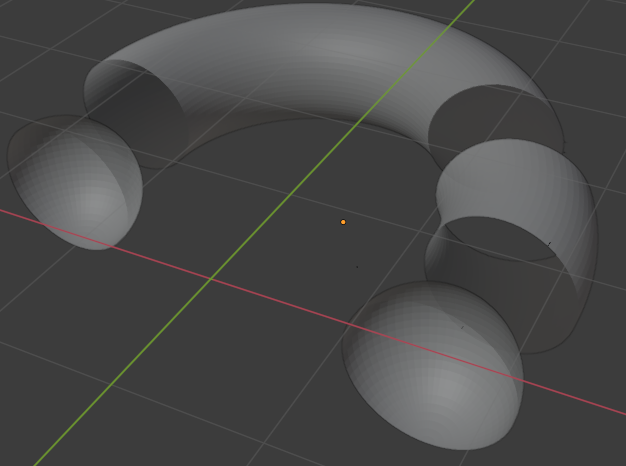
\includegraphics[width=0.36\textwidth]{fig/s16.png}} \qquad
%         \subfigure[$\partial\mathcal{Y}_2$剪开得到的曲面片]
%         {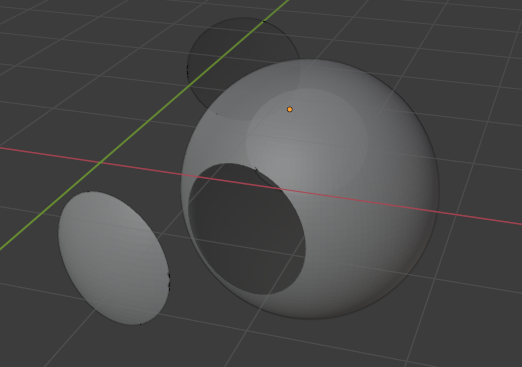
\includegraphics[width=0.375\textwidth]{fig/s17.png}}
%         %   \caption{sfd}
%         \vspace{-0.2in}
%     \end{figure}
%     \begin{figure}[!htb]
%         \centering
%         \subfigure[求交得到的殷集$\mathcal{Y}_3$]
%         {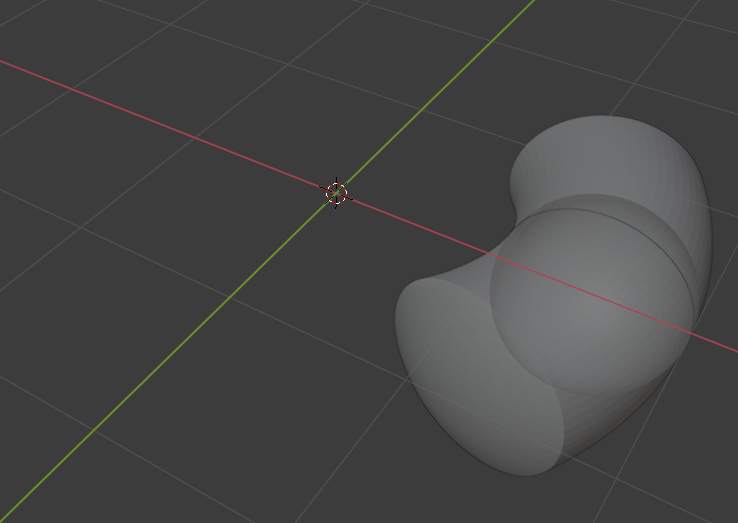
\includegraphics[width=0.35\textwidth]{fig/s5.png}} \qquad
%         \subfigure[构成$\partial\mathcal{Y}_3$的两个黏合紧曲面]
%         {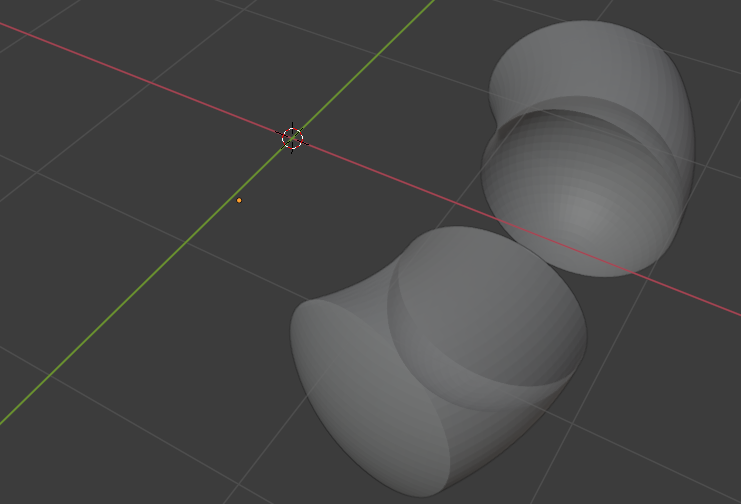
\includegraphics[width=0.365\textwidth]{fig/s6.png}}
%         %   \caption{sfd}
%         %   \vspace{0.2in}
%     \end{figure}
% \end{frame}

% \begin{frame}
%     \begin{figure}[!htb]
%         \centering
%         \subfigure[求并得到的殷集$\mathcal{Y}_4$]
%         {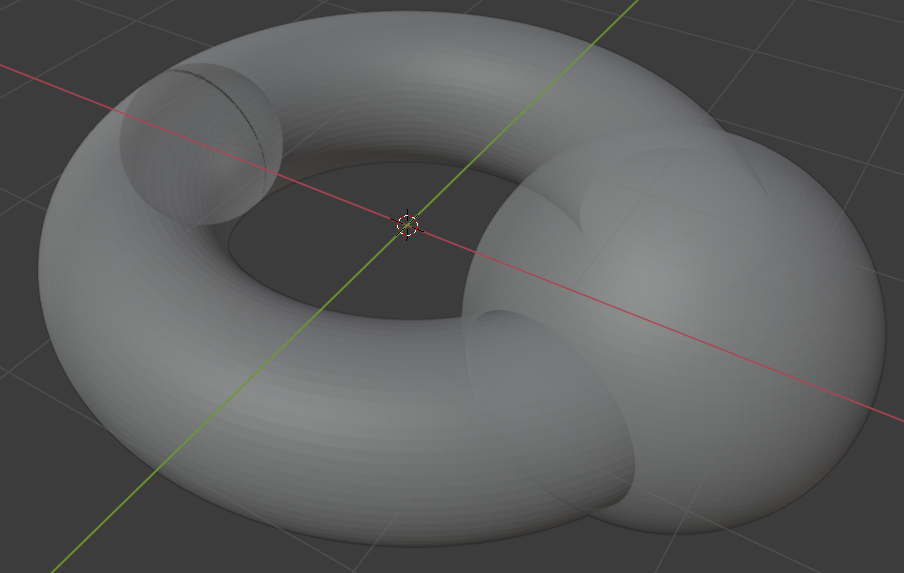
\includegraphics[width=0.35\textwidth]{fig/s7.png}} \qquad
%         \subfigure[构成$\partial\mathcal{Y}_4$的两个黏合紧曲面]
%         {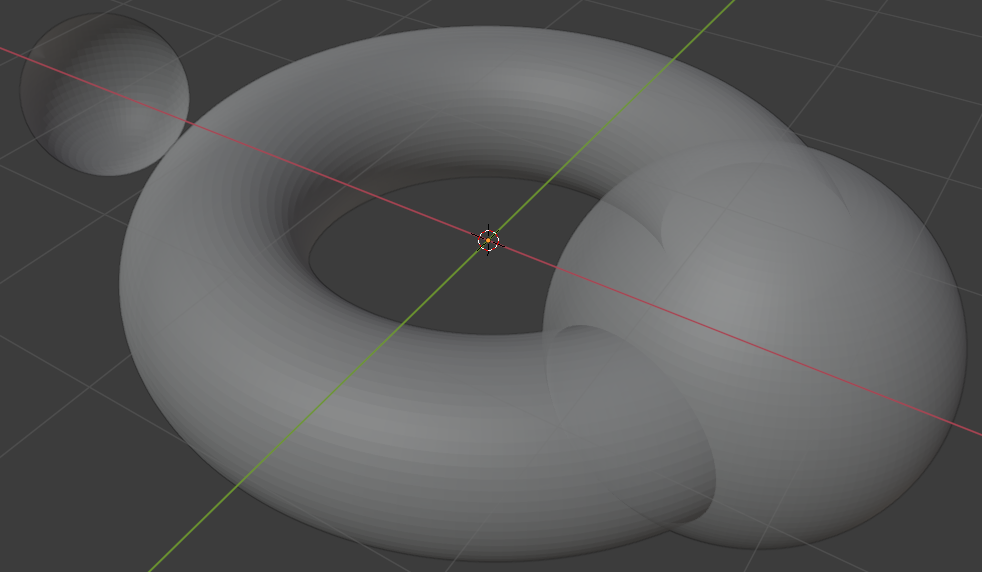
\includegraphics[width=0.365\textwidth]{fig/s8.png}}
%         \vspace{-0.05in}
%         \caption{拓扑结构复杂的殷集交并}
%         \vspace{-0.1in}
%     \end{figure}
%     \begin{figure}[!htb]
%         \centering
%         \subfigure
%         {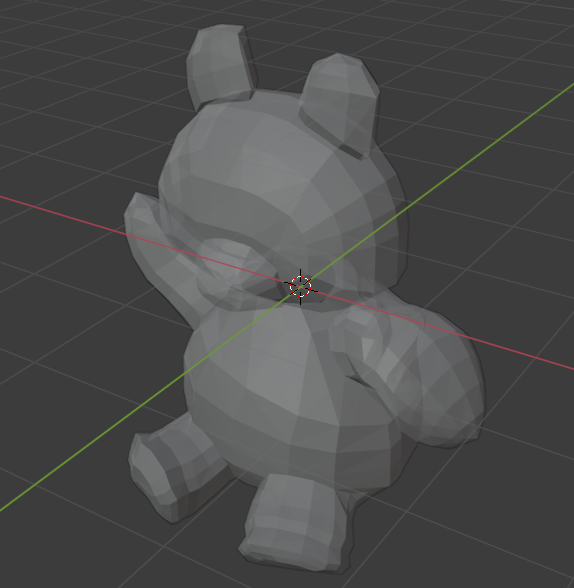
\includegraphics[width=0.27\textwidth]{fig/s10.png}} \quad
%         \subfigure
%         {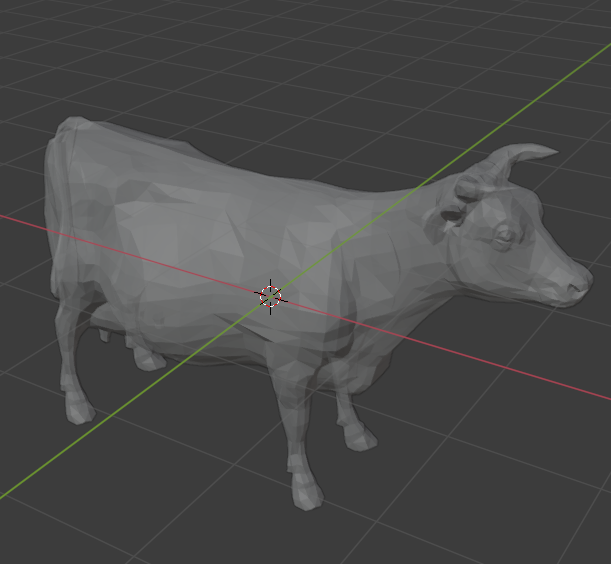
\includegraphics[width=0.3\textwidth]{fig/s9.png}} \quad
%         \subfigure
%         {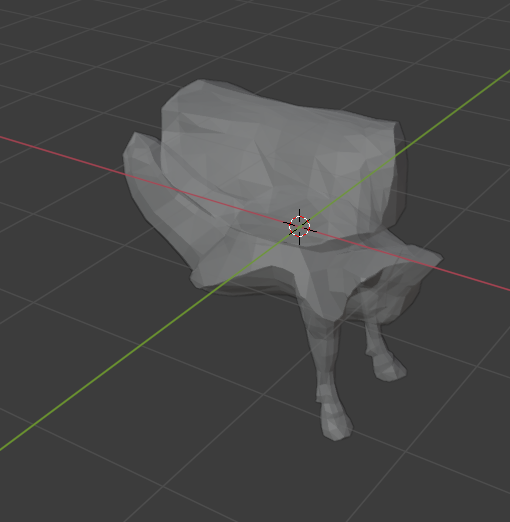
\includegraphics[width=0.27\textwidth]{fig/s11.png}}
%         \vspace{-0.05in}
%         \caption{几何特征复杂的殷集求交}
%         %   \vspace{0.2in}
%     \end{figure}
% \end{frame}

% \begin{frame}
%     \frametitle{论文在投}
%     \centering
%     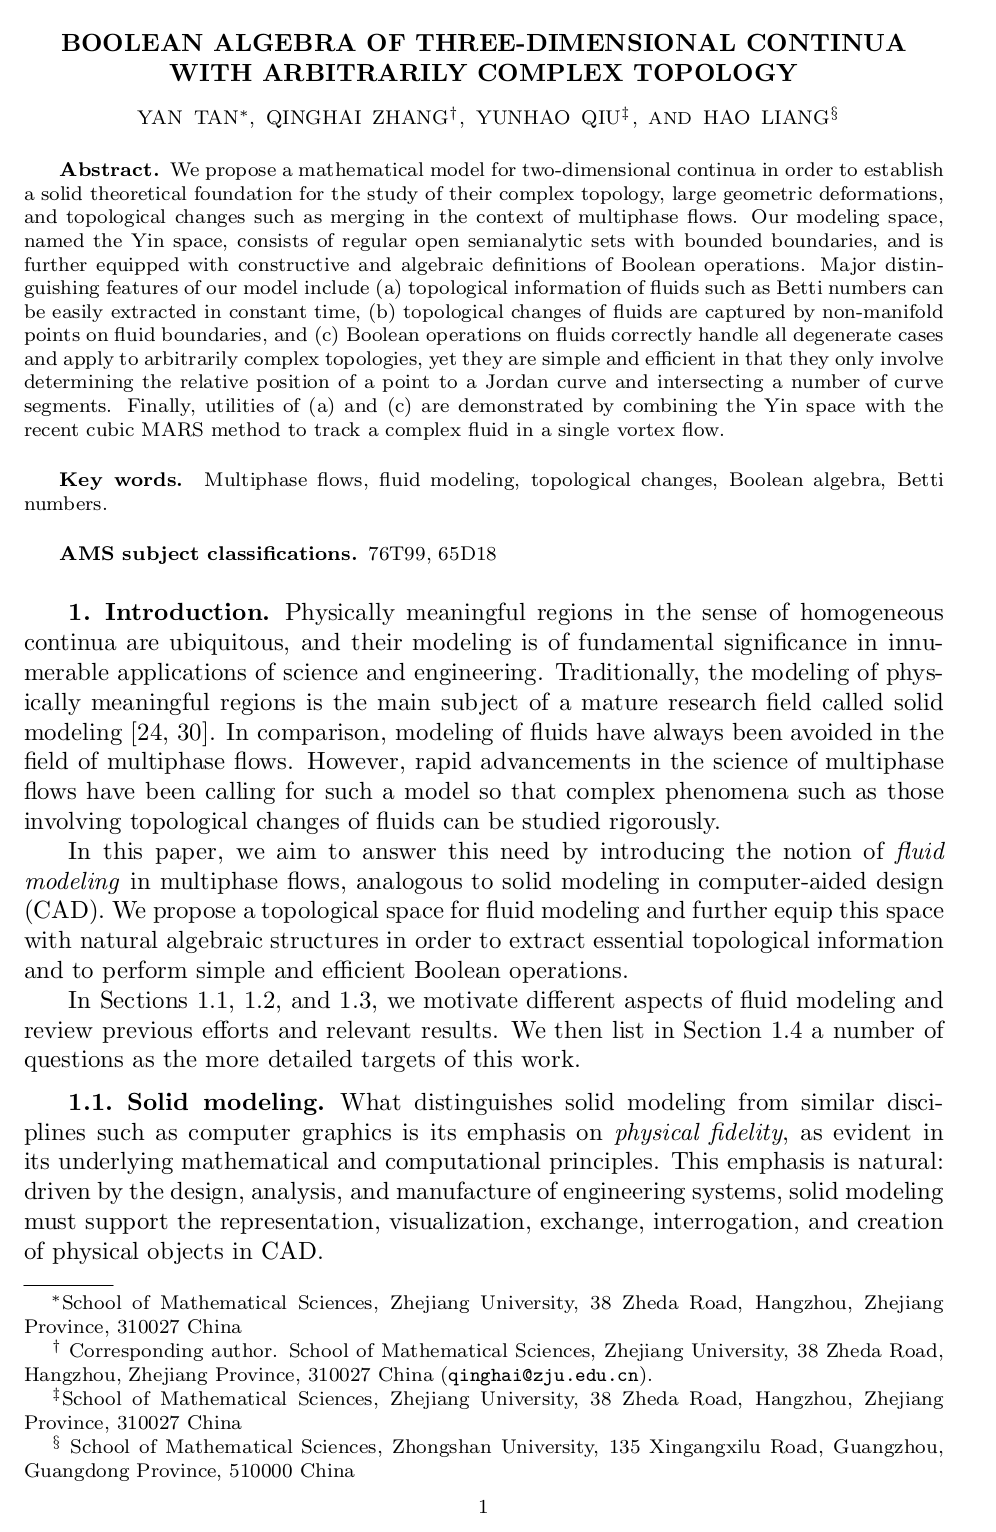
\includegraphics[height = \textheight]{fig/SIAM_Review.png}
% \end{frame}

% \section{博士阶段的研究计划}
% \subsection{流相的拓扑变化}
% \begin{frame}
%     \frametitle{博士研究计划}
%     \begin{center}
%         % \includegraphics[width = 0.7\textwidth]{fig/fig/Mars.gif};
%         \animategraphics[autoplay,
%             loop,
%             width=.5\textwidth]{5}{fig/gif/1/vortex80N64step00}{0}{62}
%     \end{center}
%     \begin{itemize}
%         \item 现有方法不能精确捕捉和刻画拓扑变化.
%         \item 结合殷集对流体建模,在MARS方法(Zhang, \tnr{ SISC}\tnrc{, \ 2018)}上
%               新增对拓扑变化的处理,并且高精度捕捉拓扑变化的时间点和位置.
%         \item 这个研究是三维殷集在军工项目中的重要应用,是项目的核心部分.
%     \end{itemize}
% \end{frame}

% \section*{}
% \begin{frame}
%     \centering\huge
%     \textcolor{red}{请各位老师批评指正!}
% \end{frame}
\end{document}